\section{Introduction}
\label{s:intro}
Vandalism is a problem encountered in content systems where the set of users permitted to edit is not restricted to a small trusted set of users. In Wikipedia, where the barrier to editing is particularly and intentionally low but the need for credibility is critical, vandalism is a big concern. Vandalism which is not promptly reverted is bad not only because it can convey misinformation and ruin the site's reputation,  but also from a security perspective, because it can even be used as a vector for other malicious attacks such as directing users via external links to phishing sites or sites containing malware.

It has been said that making a secure system against adversarial attacks is like a game of chess, not only does one have to come up with an effective strategy, but also has to counter the opponent�s response to that strategy. In our particular project, we have attempted to do the former and will discuss improvements that can be made in dealing with the latter. 

Wikipedia uses a reactive model to vandalism, rather than a preventative model. A group of users, often self-named ``patrollers'' for vandalism, scan the list of recent changes to Wikipedia, looking for suspicious changes. These users then find and revert vandalism. Vandalism detection algorithms like \sys are particularly helpful for assisting these users, as they can spot out edits which are likely to be vandalism and bring them into attention to patrollers. This way, the efforts of patrollers can be focused more on edits which are more likely to be vandalism. Vandalism detection algorithms like \sys can also revert edits automatically if it is heavily suspected of being vandalism.

Vandalism detection algorithms are not always correct. In the event of a false positive (the tool detects a legitimate edit as vandalism, and reverts it) then a user can undo the revert, in which case the algorithm will leave it as-is. In the event of a false negative (the tool fails to detect and revert actual vandalism) then the page will remain vandalized until someone else notices, and reverts it manually.


\begin{figure}[t]
\centering
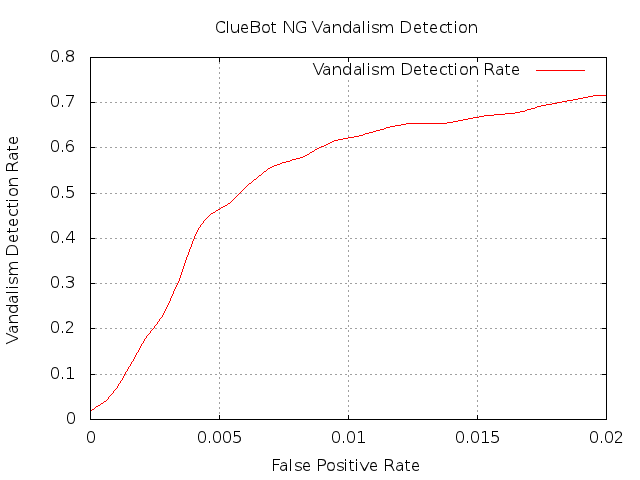
\includegraphics[width=0.7\textwidth]{figs/falsepositives-prev.png}
\vspace{-1em}
\caption{false positive rate v.s. vandalism detection rate in original \sys}
\label{f:falsepositives-prev}
\end{figure}

There are tradeoffs for each type of error; one can manipulate the threshold for declaring an edit as vandalism to reduce the number of false positives, or false negatives. In the case of \sys, the algorithm's thresholds are clearly tailored towards minimizing false positives -- the version on the sites (without our modifications) catches only 5.1$\%$ of the vandalism in the test dataset of vandalism. The particular reason for minimizing false positives is to avoid alienating users by auto-reverting their edits; new editors who have their edits auto-reverted by systems like \sys are often not aware that it was a bot which auto-reverted their edit, and can rather believe that the Wikipedia community is not welcoming of new editors, and thus stop contributing. Changing the submission and reversion process to make it more apparent and visible that algorithmic vandalism review is taking place, particularly for such new editors, may allow for a higher false positive rate to be tolerated (hence allowing more vandalism to be caught) without alienating new editors.

We define cyber vandalism as a form of activity taken up by adversaries who damage information infrastructures on the internet. There are several forms of internet vandals:

\begin{CompactItemize}
\item[1.]
Denial of Service Attacks
\item[2.]
Penetrate, hide, and collect
\item[3.]
Information Vandalism
\end{CompactItemize}

